%(BEGIN_QUESTION)
% Copyright 2011, Tony R. Kuphaldt, released under the Creative Commons Attribution License (v 1.0)
% This means you may do almost anything with this work of mine, so long as you give me proper credit

Her vises en typisk 2-leder RTD-brokrets, der RTD-en er plassert et stykke unna brokretsen:

$$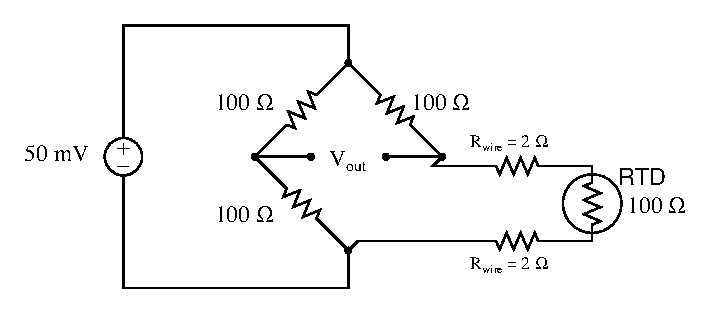
\includegraphics[width=15.5cm]{i00413x01.eps}$$

2-lederkabelen som kobler RTD-en til resten av brokretsen har resistans fordelt langs lengden. I skjemaet er dette vist i «klumpet» form som to «$R_{wire}$»-motstander. Hvilken effekt vil denne kabelresistansen ha på temperaturmålesystemet? Gir den nullpunktsforskyvning, spennviddeforskyvning eller begge deler? Hvorfor?

Beregn utgangsspenningen til denne brokretsen når 100 $\Omega$ RTD-en er ved referansetemperaturen 0$^{o}$ C, og hver $R_{wire}$-resistans er 2 $\Omega$ (hint: alpha-verdien er irrelevant i dette problemet).

Beregn også hvor varm RTD-en «ser ut» til å være ut fra brokretsens utgangsspenning når kabelresistansen legges til. Anta europeisk $\alpha$-verdi i denne beregningen.

\vskip 10pt

Her vises en typisk {\it 3-leder} RTD-brokrets, der RTD-en er plassert et stykke unna brokretsen:

$$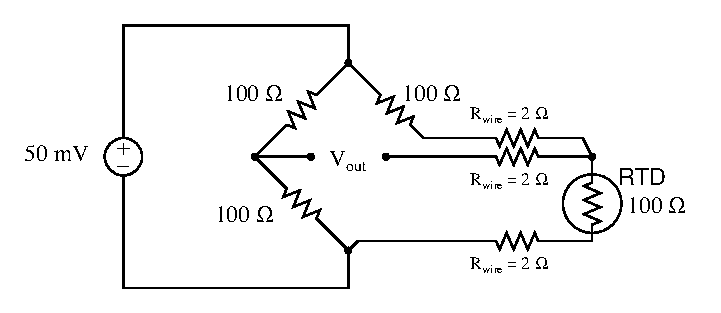
\includegraphics[width=15.5cm]{i00413x02.eps}$$

Beregn utgangsspenningen til denne brokretsen når 100 $\Omega$ RTD-en er ved referansetemperaturen 0$^{o}$ C, og hver $R_{wire}$-resistans er 2 $\Omega$ (hint: alpha-verdien er irrelevant i dette problemet):

\vskip 10pt

Kommenter hvordan denne 3-leder RTD-brokretsen sammenlignes med en 2-leder RTD-brokrets med samme kabelresistans.




\vskip 20pt \vbox{\hrule \hbox{\strut \vrule{} {\bf Forslag til sokratisk diskusjon} \vrule} \hrule}

\begin{itemize}
\item{} Forklar hvorfor RTD-ens alpha-verdi er irrelevant når temperaturen er 0$^{o}$ C.
\item{} Identifiser noen «avbruddsfeil» i en av kretsene som ville få utgangsspenningen ($V_{out}$) til å mettes «lavt» (som om RTD-en var ekstremt kald).
\item{} Identifiser noen «avbruddsfeil» i en av kretsene som ville få utgangsspenningen ($V_{out}$) til å mettes «høyt» (som om RTD-en var ekstremt varm).
\item{} En god problemløsningsmetode når vi skal finne retningen på en endring er å se på {\it grenseverdier}. I stedet for å spørre hva som skjer hvis en resistans endres litt, spør vi hva som skjer hvis resistansen endres {\it dramatisk}. Forklar hvordan denne metoden kan brukes på dette systemet.
\end{itemize}

\underbar{file i00413}
%(END_QUESTION)





%(BEGIN_ANSWER)

\noindent
{\bf Delvis svar:}

Ekstra resistans som legges inn i RTD-grenen i en 2-leder RTD-brokrets av kabellederne vil helt klart gi temperaturmålefeil, fordi RTD-en da «ser ut» til å ha høyere resistans enn den faktisk har. Dette gir en oppadgående nullpunktsforskyvning (falskt høy temperaturindikasjon).

\vskip 10pt

Denne effekten oppstår {\it ikke} i 3-leder-versjonen av brokretsen.

%(END_ANSWER)





%(BEGIN_NOTES)

For 2-leder RTD-kretsen ved 0 grader C:

\vskip 10pt

$V_{out}$ = 0.4902 mV, som tilsvarer 10.39$^{o}$ C.

\vskip 10pt

Merk: Den ekstra resistansen vil også gi en spennviddeforskyvning, og denne går også oppover (større temperaturendring kreves for å gi samme endring i utgangsspenning). For å visualisere spennviddeforskyvningen fra kabelresistans kan du tenke deg at kabelresistansen er svært stor (for eksempel 2500 $\Omega$ per leder). De ekstra 5 k$\Omega$ lagt til RTD-ens grunnresistans på 100 $\Omega$ gir 5100 $\Omega$ ved referansetemperatur. Ved høyere temperaturer vil RTD-ens ekstra resistans være svært liten sammenlignet med den totale «sløyferesistansen» i kabel+RTD-ledningene (5178.4 $\Omega$ ved 200$^{o}$ C, altså ikke stor prosentøkning fra 5100 $\Omega$ ved 0$^{o}$ C). Med andre ord «drukner» stor kabelresistans RTD-elementets egen resistans. Når prosentvis resistansendring reduseres kraftig av økt kabelresistans, blir spenningsendringen i brokretsen mye mindre enn uten lederresistans. Mindre spenningsendring for samme temperaturendring betyr redusert målespennvidde.

\vskip 10pt

Ja, det stemmer: 3-leder RTD-broen er perfekt balansert selv med ekstra lederresistans inkludert.

\vskip 10pt

Ingen beregninger er nødvendige for å løse dette problemet. Med 2 $\Omega$ resistans i hver kabelleder oppfører brokretsen seg slik:

$$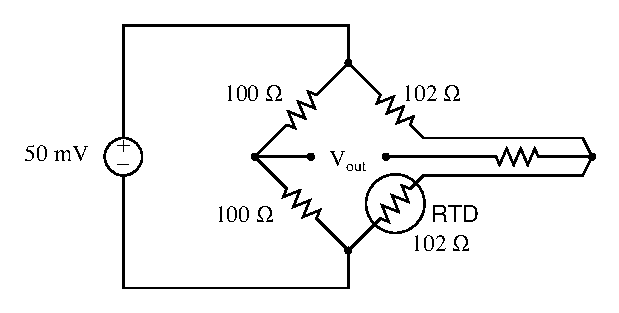
\includegraphics[width=15.5cm]{i00413x03.eps}$$

Med andre ord er dette en balansert brokrets med ekstra 2 $\Omega$ lederresistans i serie med utgangsterminalene. Vi antar et høyohmig voltmeter for måling av utgangsspenningen, og da vil 2 $\Omega$ serieresistans i voltmeterkretsen ha neglisjerbar effekt. Dessuten er utgangsspenningen 0 volt i en balansert bro uansett, så {\it enhver} serieresistans med voltmeteret ville vært uten effekt. Hvis RTD-en endrer temperatur og broen blir ubalansert, er det fortsatt viktig å forstå at 2 $\Omega$ serieresistans i linje med voltmeteret ikke vil påvirke avlesningen i nevneverdig grad, fordi voltmeteret ideelt sett ikke trekker strøm.

\vskip 10pt

Det bør likevel påpekes at en tredje leder til RTD-en ikke eliminerer alle kalibreringsfeil fra lederresistans. I tillegg til nullpunktsforskyvning når de to lederne ikke har nøyaktig samme resistans, vil det uunngåelig være en spennviddeforskyvning (en gitt endring i RTD-resistans får litt mindre effekt på brobalansen enn den ellers ville hatt).


%INDEX% Measurement, temperature: RTD (2-wire bridge with cable resistance)
%INDEX% Measurement, temperature: RTD (3-wire bridge with cable resistance)

%(END_NOTES)
